\documentclass[a4paper,12pt]{report}
\usepackage{alltt, fancyvrb, url}
\usepackage{graphicx}
\usepackage[utf8]{inputenc}
\usepackage{float}
\usepackage{hyperref}
\usepackage[italian]{babel}
\usepackage[italian]{cleveref}
\usepackage[utf8]{inputenc}
\usepackage{xcolor}
\usepackage[utf8]{inputenc}
\usepackage{titlesec}

\titleformat{\chapter}[hang] % Redefine the chapter format
  {\normalfont\huge\bfseries} % Style for the chapter title
  {} % No "Chapter" text
  {0pt} % Space between number and title
  {\thechapter\hspace{1em}} % Chapter number and title
  
\title{Progetto di IOT
    \\ SmartBin}

\author{Scorza Edoardo 0001077424 \\ Giorgini Matteo 0001136576 \\ Giuseppe Argentiere 0001089431 \\\\
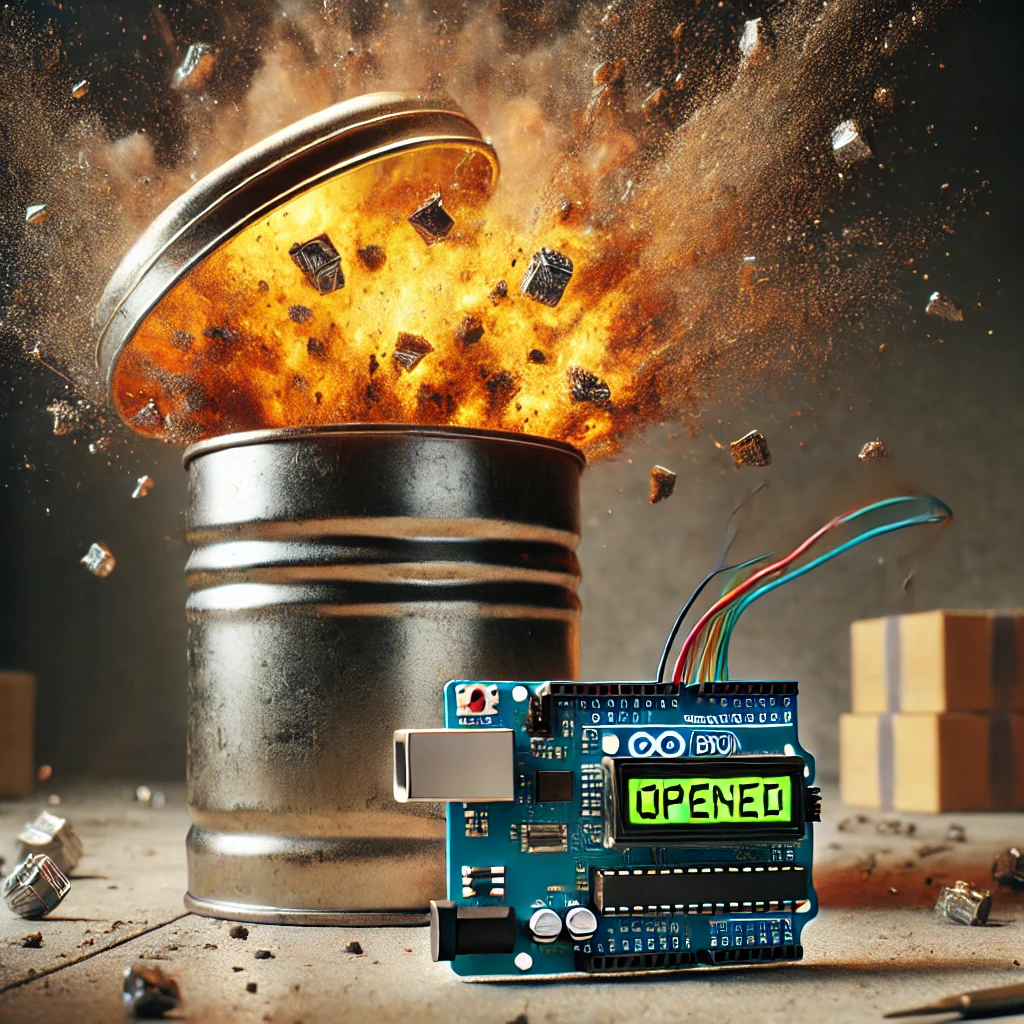
\includegraphics[width=0.5\textwidth]{images/cover.png} }
\date{1 dicembre 2024}
\begin{document}
\maketitle
\tableofcontents
\chapter{Hardware}
\begin{figure}[H] % [H] ensures the image stays exactly here
    \centering
    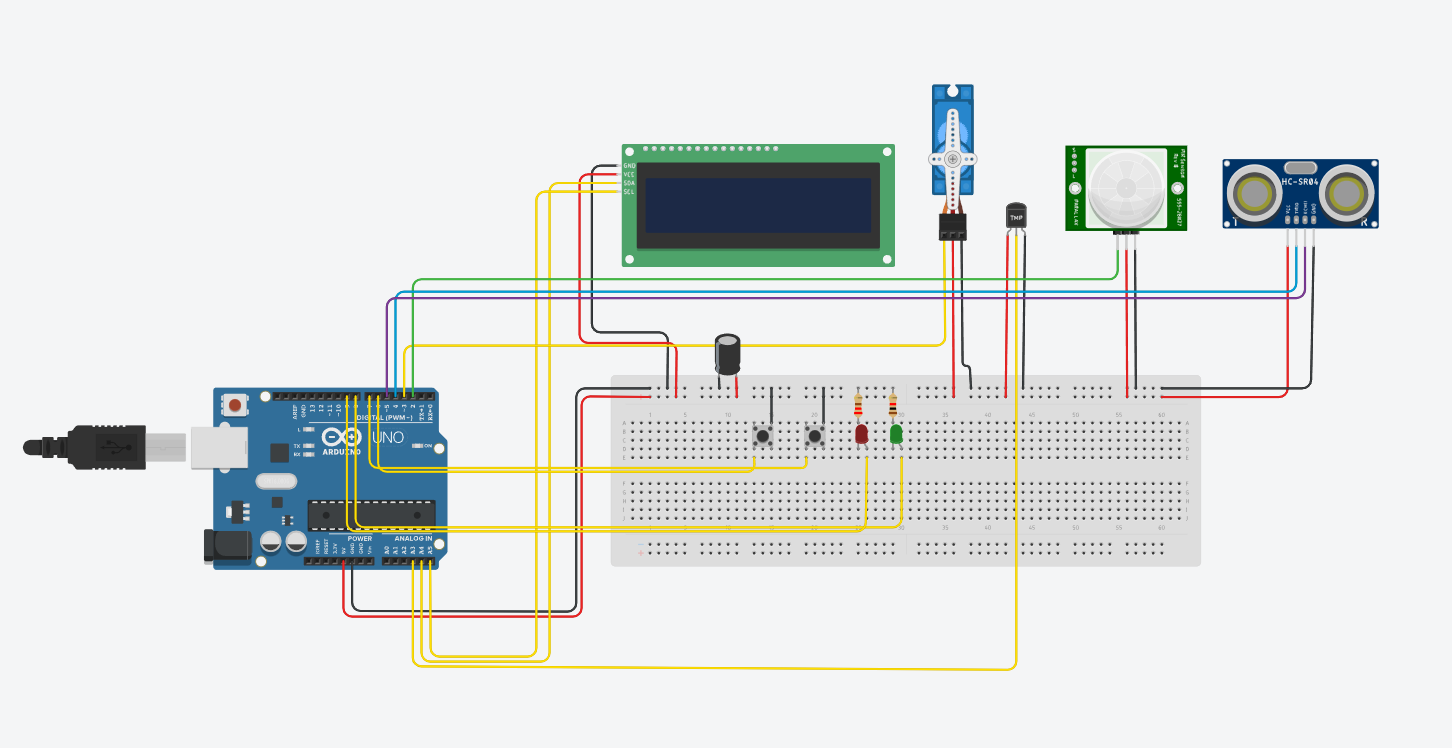
\includegraphics[width=0.8\textwidth]{images/circuito.png} % Replace 'example-image' with your file name
    \caption{Rappresentazione del circuito in Thinkercad.}
    \label{fig:sample-image} % Optional label for referencing the image
\end{figure}
\vspace{1cm}
La implementazione fisica del circuito è realizzata con i componenti 
richesti dalla specifica:
\begin{itemize}
    \item \textbf{Display LCD I2C}
    \begin{itemize}
        \item SDA: A4
        \item SCL: A5
    \end{itemize}
    \item \textbf{Button OPEN}
    \begin{itemize}
        \item Pin: 6
    \end{itemize}
    \item \textbf{Button CLOSE}
    \begin{itemize}
        \item Pin: 7
    \end{itemize}
    \item \textbf{Passive Infrared (PIR Sensor)}
    \begin{itemize}
        \item Pin: 2
    \end{itemize}
    \item \textbf{Sonar}
    \begin{itemize}
        \item Trig: 4
        \item Echo: 5
    \end{itemize}
    \item \textbf{Red LED}
    \begin{itemize}
        \item Pin: 8
    \end{itemize}
    \item \textbf{Green LED}
    \begin{itemize}
        \item Pin: 9
    \end{itemize}
    \item \textbf{Temperature Sensor (LM35)}
    \begin{itemize}
        \item Pin: A3
    \end{itemize}
    \item \textbf{Servo Motor}
    \begin{itemize}
        \item Pin: 3
    \end{itemize}
\end{itemize}
\subsection{Componenti extra}
La scelta di usare il condensatore è dato dalla presenza di 
diversi componenti e dal servo che causa picchi dovuti all'improvviso
azionamento di esso, mentre Arduino NANO è per semplificare il cablaggio del circuito.
\chapter{Software}
Per la realizzazione del software abbiamo optato per un sistema di Task e FSM,
inizialmente prevedavamo l'uso di una libreria, ma a causa del mancato supporto di Functional
ci avrebbe impedito di realizzare un oggetto con dentro la FSM.
\section{Sheduler}
Per lo Scheduler abbiamo usato la base trovata nel codice del corso e lo abbiamo 
modificato per supportare la comunicazione di Task.
\section{Task}
La classe Task è una versione modificata di quella base, con un riferimento alla propria 
variabile condivisa e un accesso a quelle delle altre Task.
\section{FSM}
Per la struttura e le specifiche richieste, la macchina a stati finiti
è stata realizzata con uno switch, nella quale sono definite transizioni, chiamate in entrata, uscita
e Timeout.
\newpage
\section{Struttura}
Il progetto è separato in varie Task, suddivise in due categorie:
\begin{itemize}
    \item \textbf{Task di Report} \\
    Queste Task si occupano di leggere e/o passare dati:
    \begin{itemize}
        \item \textbf{ButtonTask}
        \item \textbf{TemperatureTask} (FSM)
        \item \textbf{GuiTask}
        \item \textbf{WasteDetectorTask}
        \item \textbf{UserDetectorTask} (FSM)
    \end{itemize}
    
    \item \textbf{Task Decisionali} \\
    Queste Task operano sull'hardware:
    \begin{itemize}
        \item \textbf{BinTask} (FSM)
    \end{itemize}
\end{itemize}
\section{GUI}
Per la implementazione della GUI abbiamo optato per Python,
per la sua praticità e semplicità. \\
\begin{figure}[H] % [H] ensures the image stays exactly here
    \centering
    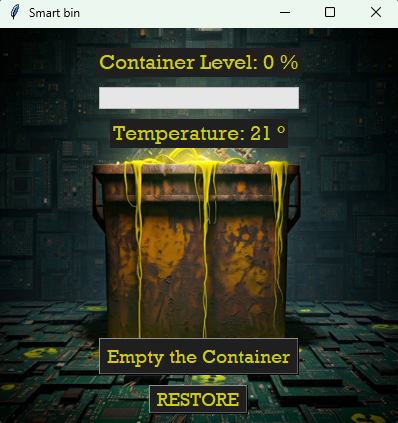
\includegraphics[width=0.5\textwidth]{images/gui.png}
    \caption{Screenshot della GUI in Python.}
    \label{fig:sample-image} % Optional label for referencing the image
\end{figure}

\subsection{Comunicazione}
Lo scambio di dati avviene mediante la \textbf{COM}.
La \textbf{ricezione} della temperatura e del livello del bidone avviene tramite testo scritto nel monitor seriale da Arduino.
Mentre la codifica della pressione dei bottoni \textbf{Empty} e \textbf{Restore} avviene tramite i caratteri \textbf{E} ed \textbf{R} stampati nel monitor seriale dalla GUI.
\end{document}